\section{Validation and case studies}

\begin{frame}
    \frametitle{Meshes for validation and performance}
    \begin{block}{Reference mesh}
		The DNS mesh for this case is a $1024^3$ DOF grid (\cite{bib:lusherTgv})
    \end{block}
    \begin{columns}
        \column{0.5\textwidth}
        \begin{table}[H]
            \centering
            \begin{tabular}{|p{1.5cm}||p{1cm}|p{2cm}|}
                \hline
                \multicolumn{3}{|c|}{Explicit case meshes} \\
                \hline
                Mesh level&Elements&Nodes\\
                \hline
                20x20x20 & 8000 & 226981\\
                40x40x40 & 64000 & 1.78e+06\\
                60x60x60 & 216000 & 5.92974e+06\\
                85x85x85 & 614125 & 1.71727e+07\\
                \hline
            \end{tabular}
            \label{table:meshPerf}
        \end{table}
        \column{0.5\textwidth}
        \begin{table}[H]
            \centering
            \begin{tabular}{|p{1.5cm}||p{1.5cm}|p{1.5cm}|}
                \hline
                \multicolumn{3}{|c|}{IMEX case meshes} \\
                \hline
                Mesh level&Elements&Nodes [M]\\
                \hline
                m1   & 31x31x31 & 2.08 \\
                m2   & 39x39x39 & 4.09 \\
                m3   & 49x49x49 & 7.96 \\
                m4   & 57x57x57 & 12.43 \\
                m5   & 88x88x88 & 43.98 \\
                \hline
            \end{tabular}
            \label{table:meshPerf}
        \end{table}
    \end{columns}
\end{frame}

\begin{frame}
    \frametitle{Validation quantities}
    \begin{itemize}
      \item Vol. Avg. Kinetic Energy: $E_k = \frac{1}{\rho_0 \Omega} \int_{\Omega} \frac{\rho}{2} u_i u_i d \Omega$
      \item Enstrophy: $\epsilon_S = \frac{1}{\rho_0 \Omega} \int_{\Omega} \mu_{eff} \left( \varepsilon_{ijk} \frac{\partial u_k}{\partial x_j} \right)^2 d \Omega$
      \item Dilational dissipation rate: $\epsilon_D = \frac{1}{\rho_0 \Omega} \int_{\Omega} \mu_{eff} \frac{\partial u_k}{\partial x_k} d \Omega$
      \item Total dissipation rate: $\epsilon_T = \epsilon_S + \epsilon_D$
      \item Maximum Mach number: $M_{max} = max( \frac{| \mathbf{u} |}{c})$
    \end{itemize}

	\begin{block}{Note on $\mu_{eff}$}
		The effective viscosity is the sum of the fluid, subgrid model and entropy viscosities: $\mu_{eff} = \mu + \mu_{sgs} + \mu_e$.
	\end{block}
\end{frame}

\begin{frame}
	\frametitle{Explicit validation: $E_k$ and $\epsilon_T$}
	\begin{figure}
		\centering
		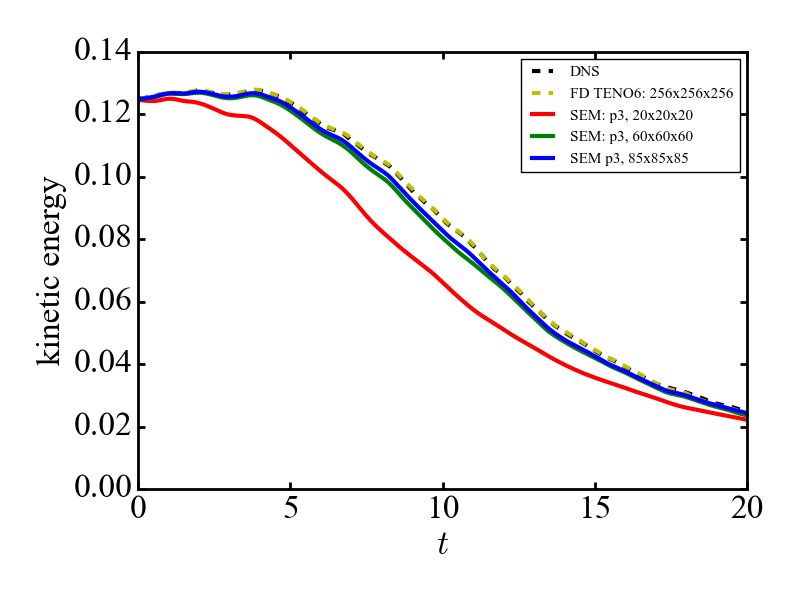
\includegraphics[width=0.49\textwidth]{images/KE.png}
		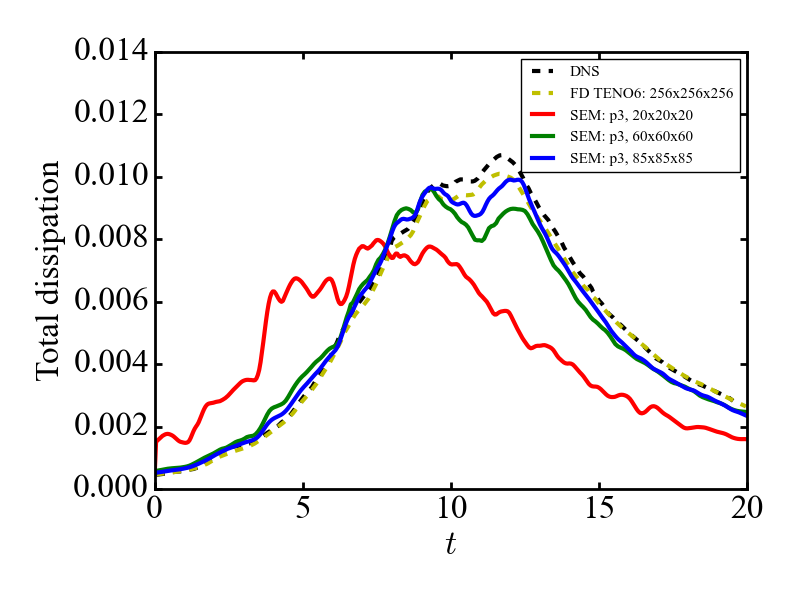
\includegraphics[width=0.49\textwidth]{images/TD.png}
        \caption{Avg. kinetic energy and total dissipation rate evolution for the explicit case meshes}
	\end{figure}
\end{frame}

\begin{frame}
	\frametitle{Explicit validation: $M_{max}$ and Mach profile}
	\begin{figure}
		\centering
		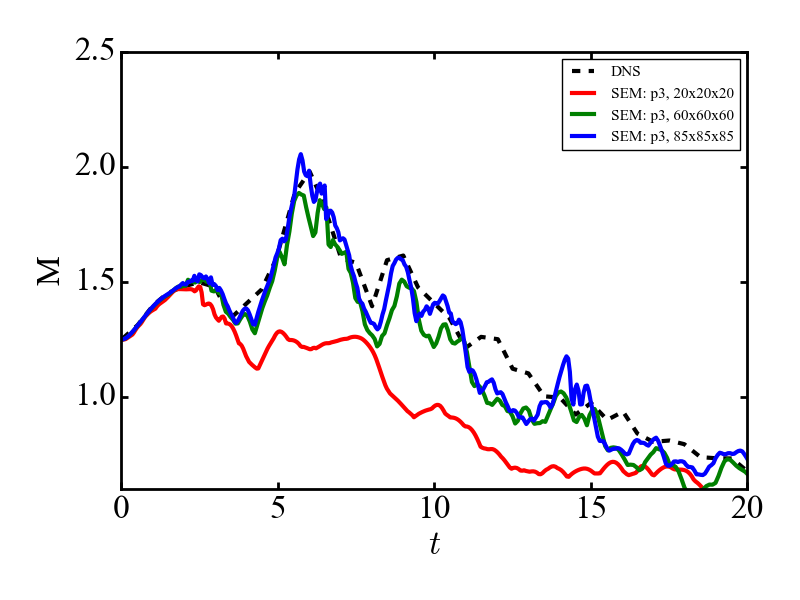
\includegraphics[width=0.49\textwidth]{images/MvsT.png}
		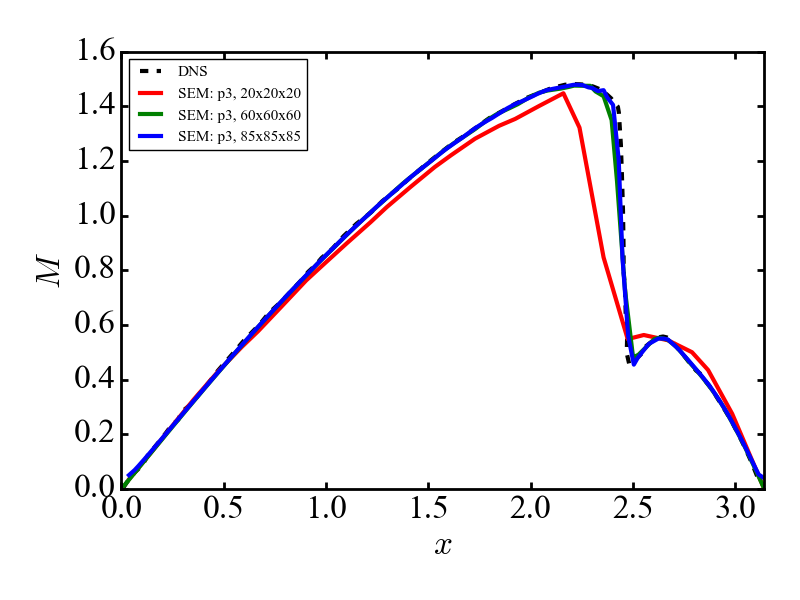
\includegraphics[width=0.49\textwidth]{images/M.png}
		\caption{Max. Mach evolution and Mach profile at plane $x = \pi$ and time $t = 2.5TU$}
	\end{figure}
\end{frame}

\begin{frame}
	\frametitle{Explicit validation: $|\nabla \rho|$ at $x = \pi$}
	\begin{figure}
		\centering
		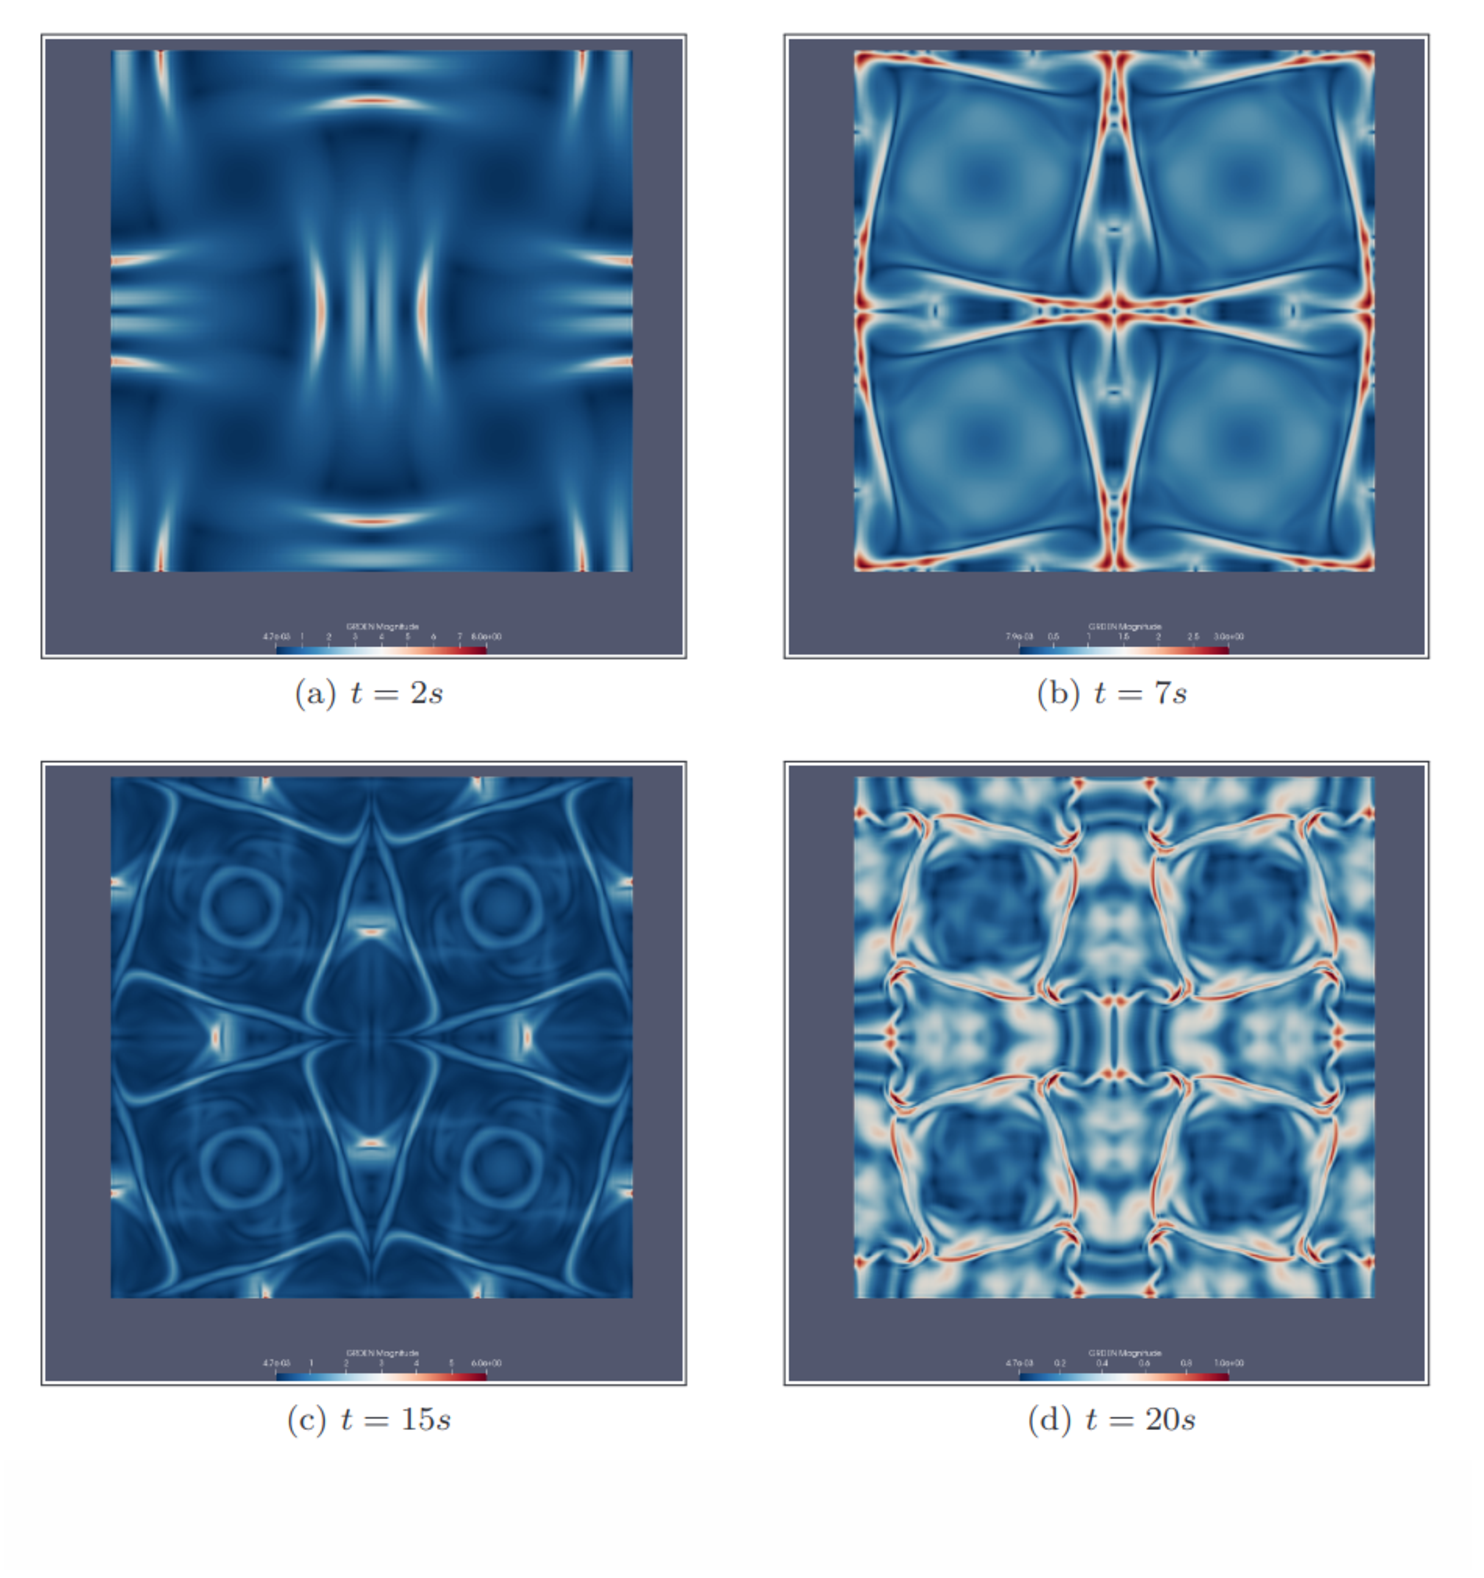
\includegraphics[width=0.6\textwidth]{images/explicitGradRho.pdf}
	\end{figure}
\end{frame}

\begin{frame}
    \frametitle{IMEX validation: $E_k$, $\epsilon_T$, $\epsilon_D$ and $M_{max}$}
    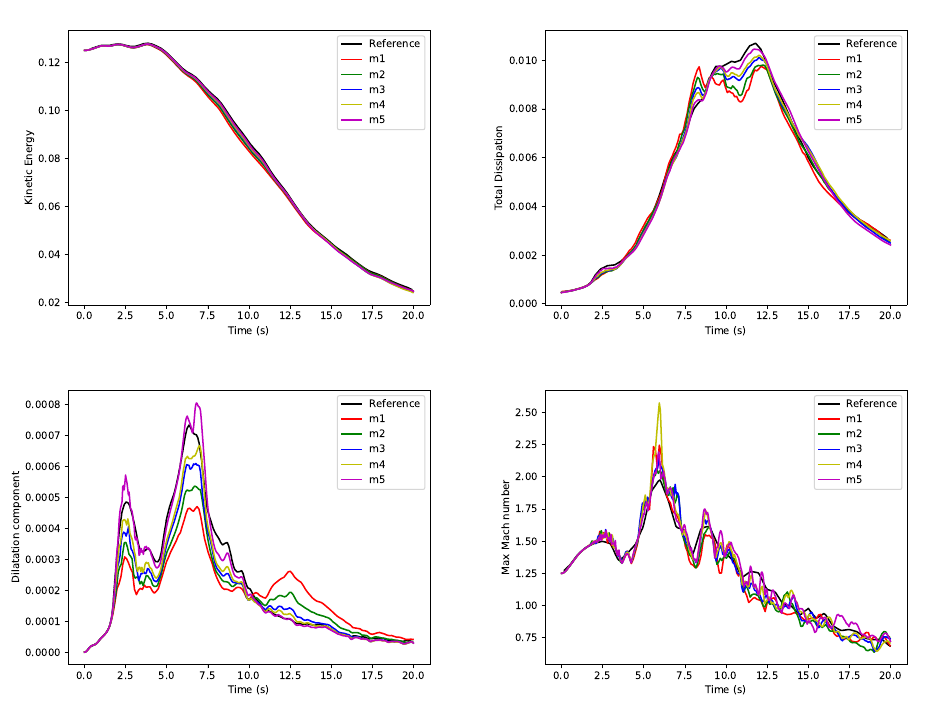
\includegraphics[width=0.84\textwidth]{images/tgv_trackers.png}
\end{frame}

\begin{frame}
    \frametitle{Fine mesh IMEX vs. RK4 comparison}
    \begin{figure}
      \centering
      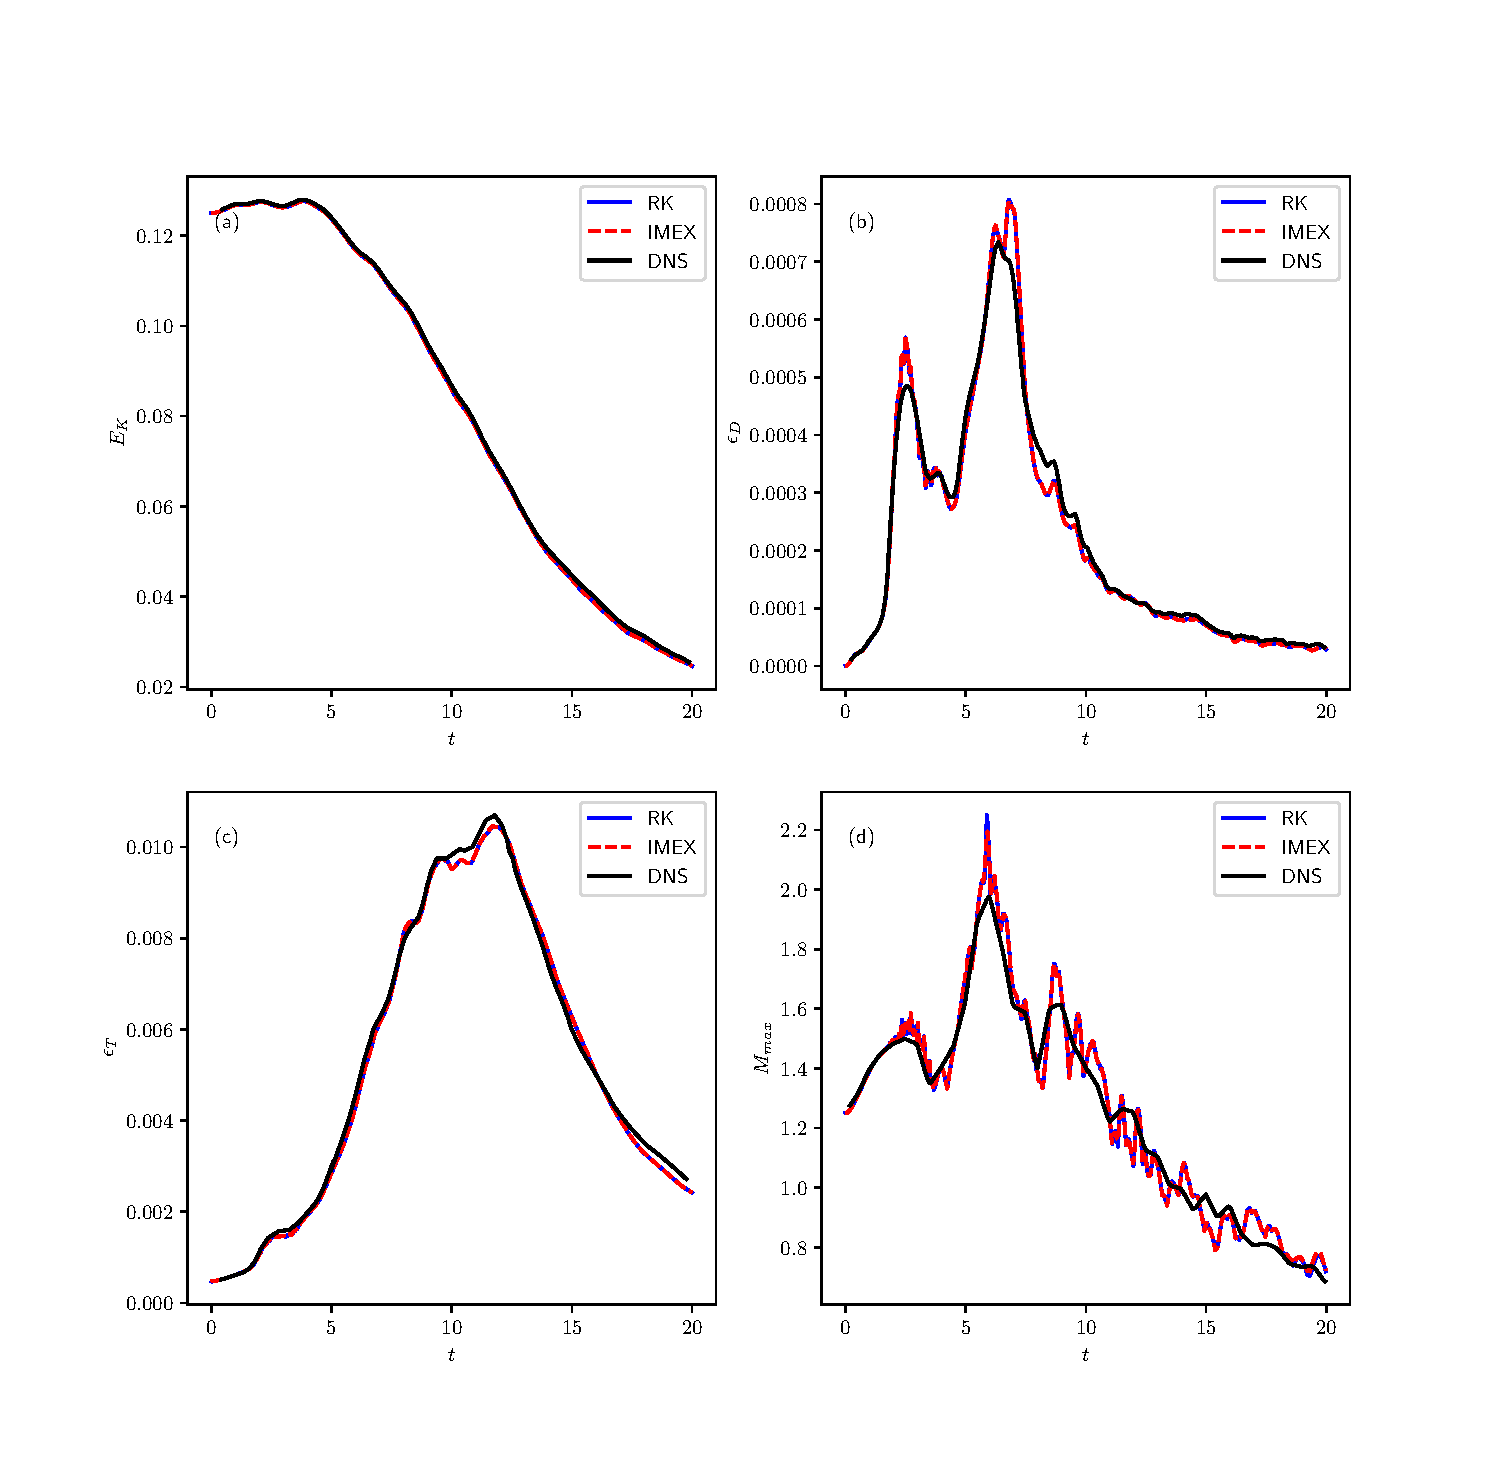
\includegraphics[width=0.7\textwidth]{images/imex_rk_comp.pdf}
    \end{figure}
\end{frame}

\begin{frame}
      \frametitle{ENVIT in action}
      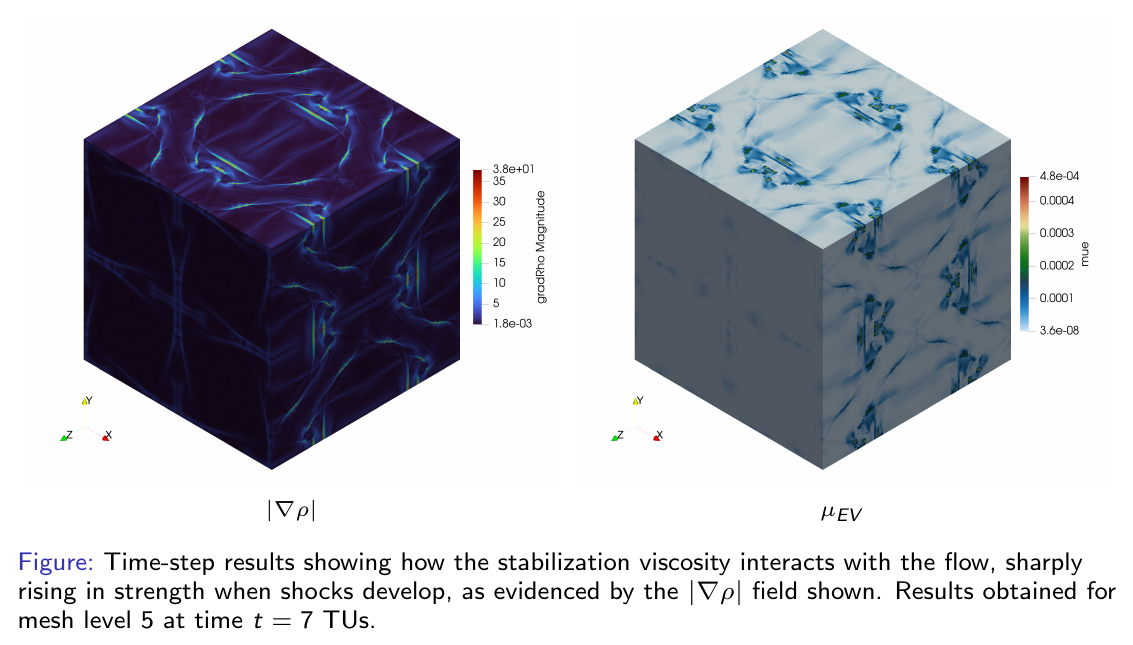
\includegraphics[width=0.96\textwidth]{images/tgv_field_t7.png}
\end{frame}

\begin{frame}
    \frametitle{Performance assessment}
    The following system configurations were utilized to measure performance:
    \begin{itemize}
      \item MareNostrum 4 node: Intel Xeon CPU, 48C at 2.2GHz (300W)
      \item Ryzen 9 CPU + NVIDIA RTX 3080Ti 12GB (400-450W)
      \item BSC CTE-POWER: IBM Power9 CPU + NVIDIA V100 16GB (300W)
      \item MareNostrum 5 ACC: Intel SapphireRapids CPU + NVIDIA H100 65GB (700W)
    \end{itemize}
    \begin{alertblock}{Important info}
      \begin{itemize}
        \item PCG converging in 1 iteration when called
        \item All GPU runs compiled using the NVIDIA NVHPC compiler suite, although versions differ
        \item Single precision floats (FP32) used whenever possible (PCG is mixed-precision)
        \item IMEX reference: explicit case using classical RK4 scheme running on the RTX 3080Ti device
      \end{itemize}
    \end{alertblock}
\end{frame}

\begin{frame}
	\frametitle{Explicit Performance results}
	\begin{table}[H]
		\centering
		\begin{tabular}{|p{2cm}||p{2cm}|p{2cm}|p{2cm}|}
			\hline
			\multicolumn{4}{|c|}{Run time of 1000 time-steps} \\
			\hline
			Mesh level&V100&RTX 3080 Ti&MN4 node\\
			\hline
			40x40x40 & 31.7s & 22.5s & 180s\\
			60x60x60 & 101.4s & 95.2s & 600s\\
			85x85x85 & 443.5s & - & 1680s\\
			\hline
		\end{tabular}
		\label{table:tstepTime}
	\end{table}
	\begin{table}[H]
		\centering
		\begin{tabular}{|p{3cm}||p{3cm}|p{3cm}|}
			\hline
			\multicolumn{3}{|c|}{Typical convective kernel runtime} \\
			\hline
			Mesh level&V100&RTX 3080 Ti\\
			\hline
			40x40x40 & 2.75ms & 1.95ms\\
			60x60x60 & 8.26ms & 6.17ms\\
			85x85x85 & 22.95mss & -\\
			\hline
		\end{tabular}
		\label{table:convKern}
	\end{table}
	
	\begin{table}[H]
		\centering
		\begin{tabular}{|p{3cm}||p{3cm}|p{3cm}|}
			\hline
			\multicolumn{3}{|c|}{Typical diffusive kernel runtime} \\
			\hline
			Mesh level&V100&RTX 3080 Ti\\
			\hline
			40x40x40 & 1.71ms & 1.25ms\\
			60x60x60 & 7.07ms & 5.57ms\\
			85x85x85 & 24.82ms & -\\
			\hline
		\end{tabular}
		\label{table:diffKern}
	\end{table}
\end{frame}

\begin{frame}
    \frametitle{IMEX Performance results}
    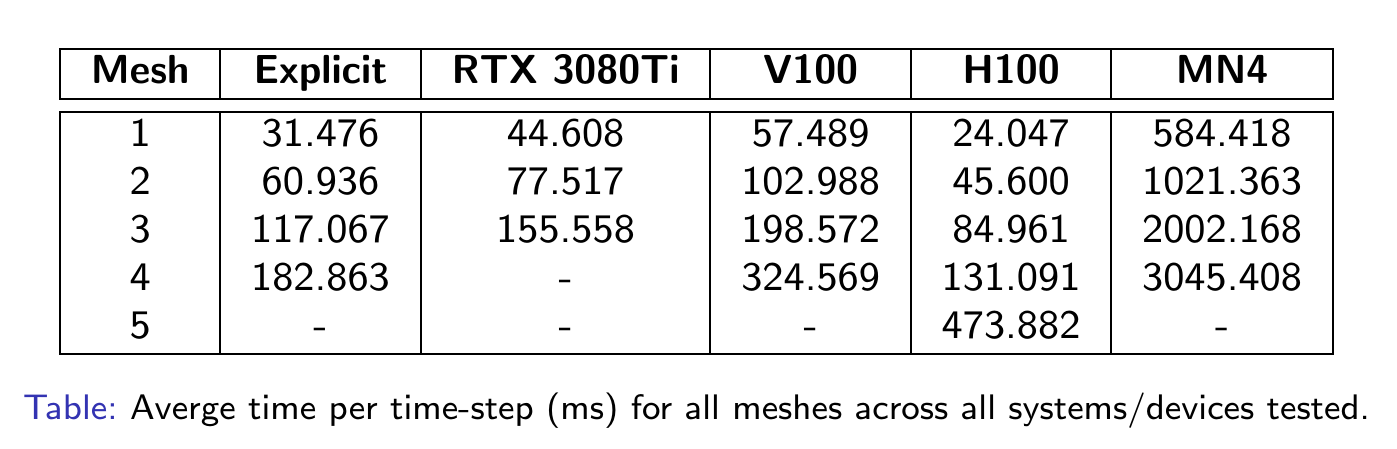
\includegraphics[width=1.0\textwidth]{images/tgv_timings.png}
    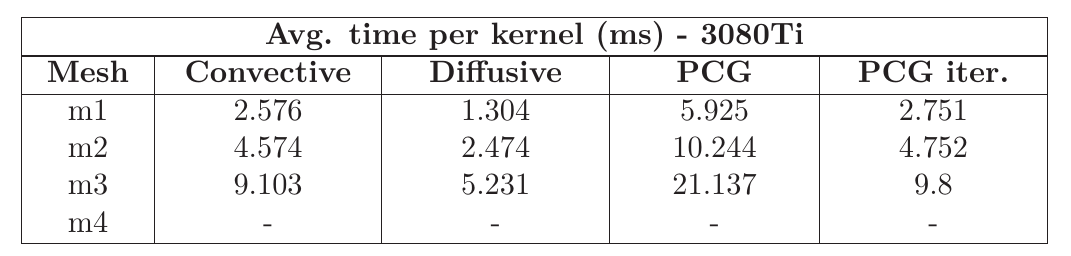
\includegraphics[width=1.0\textwidth]{images/tgv_kernels.png}
\end{frame}

\begin{frame}
    \frametitle{Compressible cylinder case}
    \begin{itemize}
      \item Studies on turbulent cylinder flow at increasing Mach numbers (\cite{bib:etmm14})
      \item $Re = 10^4$, $0.2 \leq M \leq 1.2$
      \item Wall-resolved LES, prismatic layer unstructured mesh
      \item Issues with distorted meshes $->$ explicit is a no-go
      \item Mesh: 27.5M DOFs, 3rd order hexas (64 nodes/element)
    \end{itemize}
    \begin{block}{Remark}
    On severly distorted elements, the stabilizing entropy viscosity experiences sharp rises that either force an unfeasible time-step (dominant diffusive CFL) or lead to solution divergence.
    \end{block}
\end{frame}
    
    \begin{frame}
    \frametitle{Cylinder results}
    
    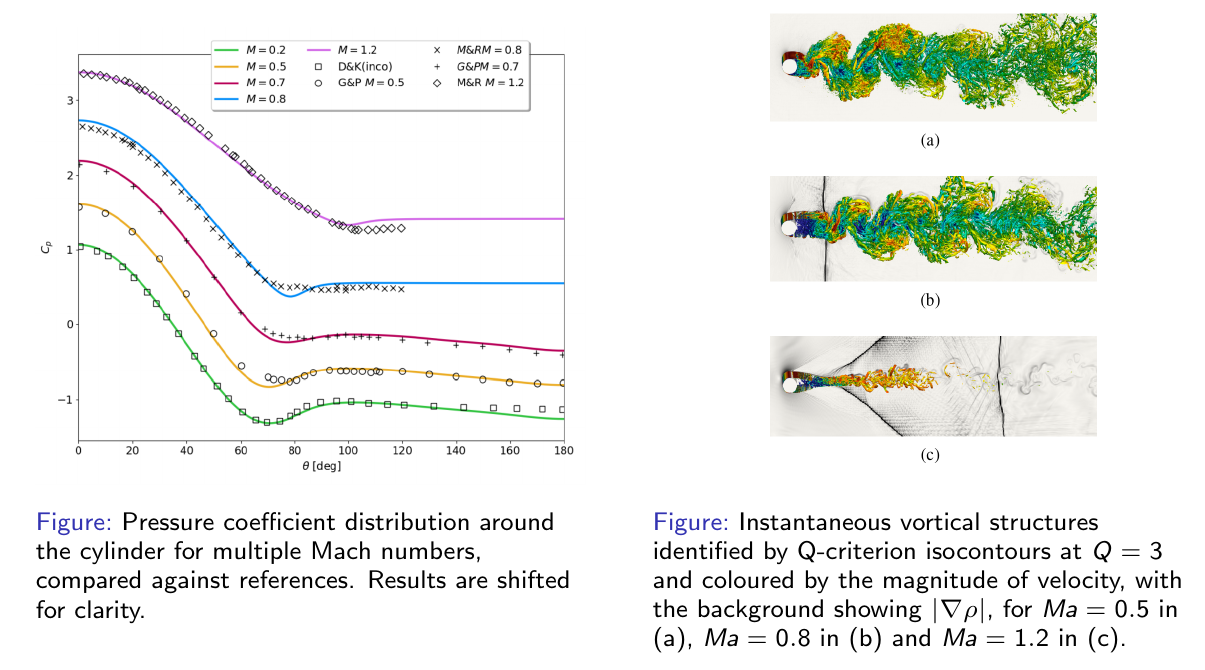
\includegraphics[width=1.0\textwidth]{images/cylinder_results.png}
    \end{frame}
    
    \begin{frame}
    \frametitle{NASA High-Lift Prediction Workshop 5 (HLPW5)}

    \begin{itemize}
      \item High-Lift Common Research Model (CRM-HL) (\cite{bib:crm})
      \item Case 2.4: Wing-Body-Slat-Flaps-Nacelle with HV
      \item Free-stream Mach: $M = 0.2$
      \item Resolved with IMEX (transients) + ERK (steady state)
    \end{itemize}
    
    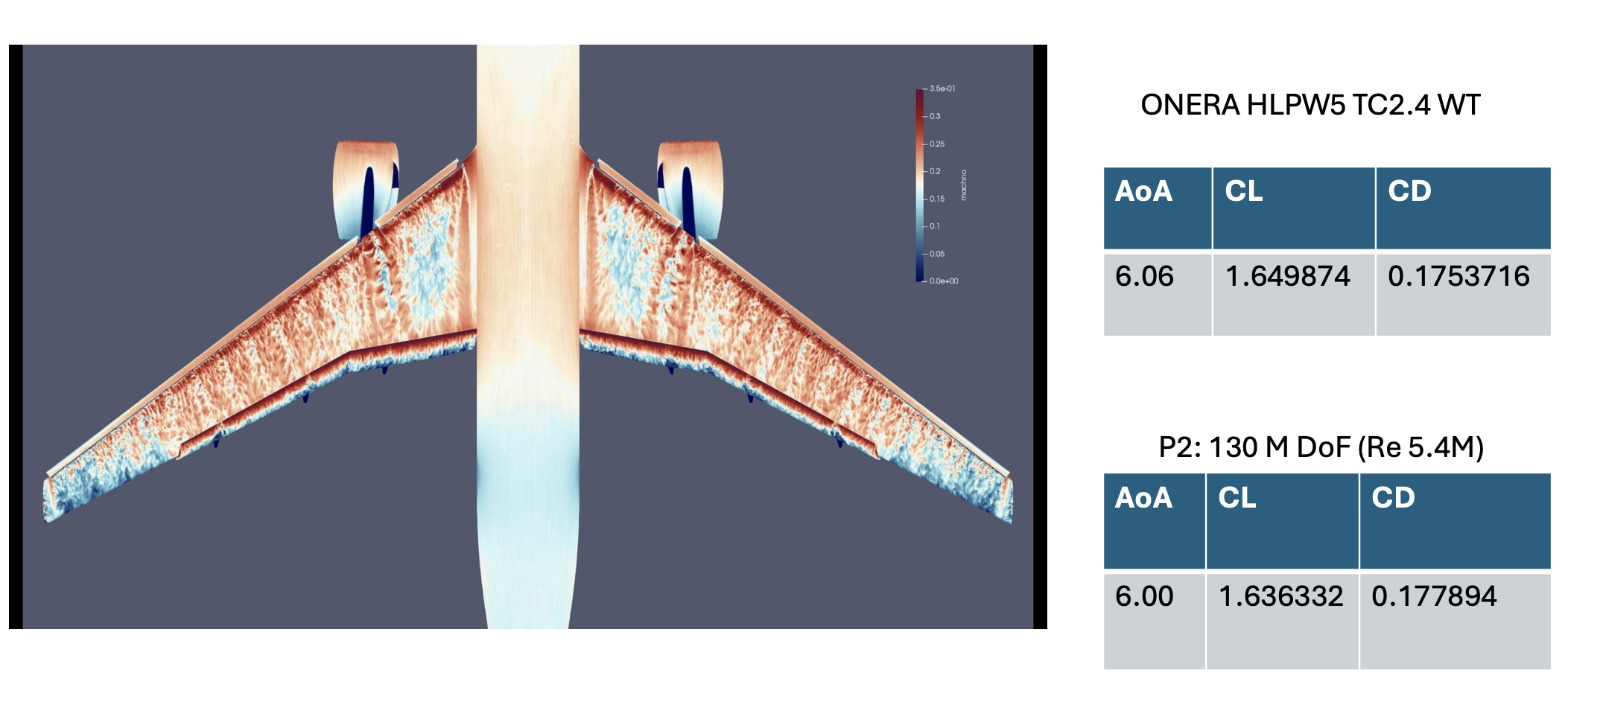
\includegraphics[width=1.0\textwidth]{images/crm.png}
    
    \end{frame}